\linespread{1.11}\selectfont

%%%%%%%%%%%%%%%%%%%%%%%%%%%%%%%%%%%%%%%%%%%%%%%%%%%%%%%%%%%%%%%%%%
%%%%%%%%%%%%%%%%%%%%%%%%%%%%%%%%%%%%%%%%%%%%%%%%%%%%%%%%%%%%%%%%%%
\chapter{Методы моделирования временных рядов}
%%%%%%%%%%%%%%%%%%%%%%%%%%%%%%%%%%%%%%%%%%%%%%%%%%%%%%%%%%%%%%%%%%
%%%%%%%%%%%%%%%%%%%%%%%%%%%%%%%%%%%%%%%%%%%%%%%%%%%%%%%%%%%%%%%%%%
\section{Статистические методы и средства анализа рядов}
Для прогнозирования будущих показателей имеющегося временного ряда   необходимо построить модель ряда,  которая наиболее полно отражает изменение  исследуемого ряда. Существует множество  моделей, описывающих различные  стохастические процессы и имеющие  различные формы представления, но среди  них выделяют следующие, имеющие наибольшую  ценность в практике:
\begin{itemize}
\item авторегрессионные модели (первого порядка, второго порядка)- \\(Autoregressive Moving Average, ARMA);
$$
	y(t)=c + \sum _{i=1}^{p} {a_i  y(t-i)} + \epsilon_t
$$

\item модели скользящего среднего (Moving Average);
$$
	\bar y(k) = \frac {1} {n} \sum _ {t=k} ^ {n+k} {y(t)}
$$

\item интегральные модели (Autoregressive Integrated  	Moving Average, ARIMA);
$$
	\Delta ^ d y(t)=c + \sum _{i=1} ^{p} {a_i  \Delta ^ d y(t-i)} + \frac {1} {q} \sum _{j=1} ^{q} {b_j \Delta ^ d y(t-j)} + \epsilon_t
$$
\end{itemize} 

В целом, статистический подход к анализу временных рядов заключается в выявлении и моделировании его детерминированных компонент на основе аддитивной (или мультипликативной) параметрической функциональной модели, приведении остатков к стационарному виду, при моделировании которых полученные ошибки удовлетворяли ограничениям модели

Изучение временных рядов осуществляется при помощи вероятностно-статистических моделей. При этом выделяют характеристики временного ряда $x(t)$:
\begin{itemize}
\item математическое ожидание $a(t) = Mx(t)$;
\item дисперсия $\sigma^2(t) = Dx(t)$;
\item автокорреляционая функция временного ряда: 

$p(t,s) = \frac{M(x(t)-a(t))(x(s)-a(s))}{\sigma(t)\sigma(s)}$.
\end{itemize}
В зависимости от значений этих показателей временные ряды делятся на стационарные и нестационарные.

Стационарные временные ряды можно выделить с помощью такого критерия как неизменность ранее перечисленных характеристик временного ряда: математическое ожидание и дисперсия являются постоянными величинами, автокорреляционная функция зависит только от разности $t-s$. Иначе временной ряд является нестационарным.

Нестационарные временные ряды.
В терминах статистики в поведении временного ряда обычно выявляют две основные тенденции -- тренд и периодические колебания. При анализе временных рядов стараются выделить тренд. Если затем вычесть его из исходных данных то остается колеблющийся ряд - случайные скачки, нерегулярности. Существенным понятием для тренда является гладкость.  
Представляются следующие методы представления тренда:
\begin{itemize}
\item функциональная форма, полином низкой степени; 

	плюсы:
	простая форма представления;

	недостатки:
	\begin{itemize}
		\item трудно производить обновление,
		\item сложно оценивать параметры функции,
		\item подбор новой функции после добавления новых точек ряда может исказить полученную ранее последовательность.
	\end{itemize}
\item скользящие средние; 

	плюсы: упрощенная форма полиномиального представления;

	минусы: возможность сгладить циклическую, краткосрочную составляющую тренда, запаздывание значений относительно исходного ряда;

\item взвешенные скользящие средние;

	плюсы: учитывается расстояние от точки до середины интервала сглаживания;

	минусы: усиливает зависимость уровней ряда друг от друга;

\item экспоненциальная средняя;
	%вставить формулу%

	плюсы: влияние прошлых наблюдений затухает по мере удаления от момента, для которого определяется средняя;

	минусы: влияние будет значительным для первых членов ряда, следовательно ряд должен иметь достаточно большое количество уровней;

	условия применения: наличие предыдущего значения в связи с рекурентным процессом вычисления;
	выбор оптимальной постоянной сглаживания, характеризующей скорость реакции модели на изменение уровней.

\end{itemize}

Главный недостаток этих методов в том, что они рассматривают временной ряд изолированно от других явлений,
и если даже имеется дополнительная информация, она может быть использована исследователем лишь путем регулирования скорости адаптации. Кроме того, точность прогнозов заметно падает при долгосрочном прогнозировании. 

Следующим шагом после сглаживания тренда является моделирование стационарного процесса - разности между трендом и временным рядом. Такие ряды составляют другой класс временных рядов (в отличие от рядов, для которых возможно применить сглаживание с помощью скользящего среднего с конечным отрезком усреднения) , известный как класс авторегрессий. <<К данному ряду можно относиться как к генерируемому механизмом, в котором значение ряда в момент времени t  выражается через прошлые значения - систематическая зависимость от прошлой истории плюс случайная погрешность>>.

%этапы построения моделей%

Минусы стационарных моделей:

Не существуют однозначных и эффективных критериев и методов определения факта наличия детерминированного тренда. Существуют статистические критерии проверки гипотезы о наличии тренда. Но эти критерии используют двухальтернативный базис: тренд или случайная компонента (метод восходящих-нисходящих серий), тренд или периодическая компонента, регулярная или случайная компонента.

Статистические модели характеризуются невысоким качеством при моделировании коротких временных рядов (количество наблюдений меньше 40)

Минусы статистических методов:
\begin{itemize}
\item отсутствие в модели представлений о структуре и системе связей реального объекта, что вносит субъективизм в выбор как самой модели, так и ее структуры;
\item трудность построения моделей при условии, что данные хранятся в разных временных рядах и (или) имеют временные сдвиги относительно друг друга;
\item значительная чувствительность получаемых результатов к недостатку информации и (или) ее зашумленности;
\item потребность в высокой квалификации математиков-программистов;
\item зависимость результата прогноза от квалификации аналитика в конкретной предметной области. 
\end{itemize}

\section{Нейросетевые методы и средства анализа рядов}
Последняя тенденция - сочетание линейных и нелинейных моделей для прогнозирования временных рядов является активной областью исследований. 

Гибкость и силовые возможности нейронных сетей  применительно к распознаванию сделали их привлекательной альтернативой, когда структура данных порождающей системы неизвестна. Однако, если начать формулировать прогностическую модель, ИНС, как правило, трудно интерпретировать и для проверки статистической значимости параметров. .

Нейронные сети благодаря своим свойствам хорошо зарекомендовали себя при обработке данных. Одной из важных особенностей является способность к обучению и обобщению накопленных знаний. На ограниченном множестве данных сеть, обобщая полученную информацию, показывает хорошие результаты на данных, которые не использовались при обучении.
Функции, выполняемые сетями:
\begin{itemize}
\item аппроксимация,
\item классификация и распознавание образов,
\item прогнозирование,
\item идентификация и оценивание,
\item ассоциативное управление.
\end{itemize}

<<В каждом из названных приложений нейронная сеть играет роль универсального аппроксиматора функции от нескольких переменных, реализуя нелинейную функцию $y=f(x)$, где x - входной вектор, y - реализация векторной функции нескольких переменных.>> Постановки значительного количества задач моделирования могут быть сведены именно к такому представлению.
<<Для классификации и распознавания образов сеть обучается важнейшим их признакам, таким, как геометрическое отображение конечной структуры изображения, относительное расположение важнейших элементов образа, компоненты преобразования Фурье и другие подобные факторы. В процессе обучения выделяются признаки, отличающие образы друг от друга, которые и составляют базу для принятия решений об отнесении образов к соответствующим классам.>> 

<<При решении задач прогнозирования роль нейронной сети состоит в предсказании будущей реакции системы по ее предшествующему поведению. Обладая информацией о значениях переменной $x$ в моменты, предшествующие прогнозированию $x(k-1), x(k-2), ..., x(k-N)$, сеть вырабатывает решение, каким будет наиболее вероятное значение последовательности $\widehat{x}(k)$ в текущий момент $k$>>.

<<Моделирование ВР в рамках нейросетевого подхода сводится к задаче наилучшей аппроксимации нелинейной функции от многих переменных по набору примеров, заданных историей временного ряда:
$$\widehat{y}_{k+1}=\phi(y_k, ..., y_{k-n+1}) + \epsilon_{k+1} $$
где $\widehat{y}_{k+1}$ - прогнозируемое значение уровня временного ряда; \\
$y_k, ..., y_{k-n+1}$ - наблюдаемые значения уровней временного ряда;\\
$\phi(y_k, ..., y_{k-n+1})$ - некоторая нелинейная функция, параметрической моделью которой служит нейронная сеть;
$\epsilon_{k+1}$ - ошибка прогноза;
$n$ - порядок модели>>.

Эффективность нейронной сети во многом зависит от ее структуры. Взаимодействие между различными узлами сети
задаются с помощью структуры. Структура ИНС не является уникальной для данной задачи, и могут существовать различные способы определить структуру, соответствующую проблеме. В зависимости от задачи, может оказаться целесообразным иметь больше одного скрытого слоя, упреждающие или обратные связи, а в некоторых случаях, прямые связи между входным и выходным слоем.

Успех нейросетевого моделирования зависит от
\begin{itemize}
\item типа данных;
\item умения аналитика в выборе подходящей нейросетевой модели и / или;
\item численных методов, используемых в модели и для вычисления прогнозов.
\end{itemize}
Исследования показали, что хорошая модель нейросетевая модель для временных рядов должна быть выбрана путем сочетания традиционного моделирования со знанием анализа временных рядов и проблем, связанных с параметрами нейросетевых моделей.  

Влияние на качество нейросетевой модели оказывает также размер окна -  количество данных, участвующих в прогнозе.
Если окно слишком мало, то аттрактор системы проецируется на пространство недостаточной размерности. Кроме того, окно слишком большого размера может привести к проблемам: кроме основной информации в окно попадает шум.

Выделяется три сущности, необходимые для построения нейронной сети:
\begin{enumerate}
\item Модель нейронной сети, архитектуры.
\item Алгоритм обучения, который определяет веса связей.
\item Функция, которая определяет выход каждого нейрона, функция активации.
\end{enumerate}
Модели нейронной сети могут быть разделены
на следующие три типа:
\begin{enumerate}
	\item Сети c прямой связью: рассматривают восприятие
моделью обратного распространения, в основном используется в таких областях, как прогнозирование
и распознавания образов;
	\item Сети с обратной связью: в основном используется для
ассоциативной памяти и оптимизации расчетов;
	\item Самоорганизующиеся сети: рассматривают модели адаптивной
резонансной теории и модели Кохонена, используется для кластерного анализа
\end{enumerate}

Ниже в таблице \ref{table:neuro_stat_compare} мы перечислим сопоставимые свойства, взятые из теории 
нейронных сетей и статистических методов:

\begin{table}[!h]
\caption{}
\label{table:neuro_stat_compare}
\begin{center}
\begin{tabular}{|p{0.4\linewidth}|p{0.4\linewidth}|}
\hline \textbf{Нейронная сеть} & \textbf{Статистика} \\
\hline Функции: & переменные \\
\hline входы & независимые переменные \\
\hline выходы & спрогнозированное значение \\
\hline цели или значения для обучения & зависимые переменные \\
\hline ошибки & остатки \\
\hline обучение & расчет \\
\hline функция ошибок & оценочный критерий \\
\hline образцы или пары обучения & наблюдения \\
\hline (синаптические) веса & оценки параметров \\
\hline нейроны высокого порядка & взаимодействия \\
\hline функциональные связи & преобразования \\
\hline обучения с учителем & регрессии и дискриминантный анализ \\
\hline неконтролируемое обучение & сжатие данных \\
\hline конкурентного обучения или кластерный анализ & адаптивный вектор квантования \\
\hline обобщение & интерполяции или экстраполяции \\
\hline
\end{tabular}
\end{center}
\end{table}

В настоящее время нейронные сети наиболее часто используются при интеллектуальном анализе данных
временных рядов. 
Преимущества применения нейронных сетей:
\begin{itemize}
	\item высокая точность: нейронные сети могут аппроксимировать сложные нелинейные отображения;
	\item устойчивость к шуму: нейронные сети являются очень гибкими по отношению к неполным, пропавшим и зашумленным данным;
	\item независимость от предыдущих предположений: нейронные сети не делают априорных предположений о 
	распределении данных или формы взаимодействия между факторами;
	\item простота обслуживания: нейронные сети могут быть использованы с новыми данными, что делает их полезными в динамических средах;
	\item могут быть реализованы в параллельном оборудовании;
	\item когда элемент нейронной сети выходит из строя, она может продолжать работать без каких-либо проблем.
\end{itemize}

Возникающие проблемы:
\begin{itemize}
 \item нет общих методов для определения оптимального количества нейронов, необходимого для решения любой задачи;
 \item трудно выбрать набор обучающих данных, который будет достаточен для решения задачи.
\end{itemize}

Искусственные нейронные сети имеют как общие проблемы, такие как сходимость, устойчивость, наличие минимальных параметров настройки, так и частные проблемы анализа временных рядов: малая скорость обучения, попадание в локальный минимум, трудность определения параметров тренировки.
Объединение генетических алгоритмов с нейронными сетями помогают достичь более высоких результатов.

\section{Методы и средства интеллектуального анализа данных}

Интеллектуальный анализ данных процесса может быть составлен на три основных этапа:
подготовка данных, интеллектуального анализа данных, выражения и интерпретации
результатов. Интеллектуальный анализ данных это итерационный процесс повторения этих трех фаз. 
Детали показаны на рис. \ref{pict:datamining1}.

\begin{figure}[h!]
\center
	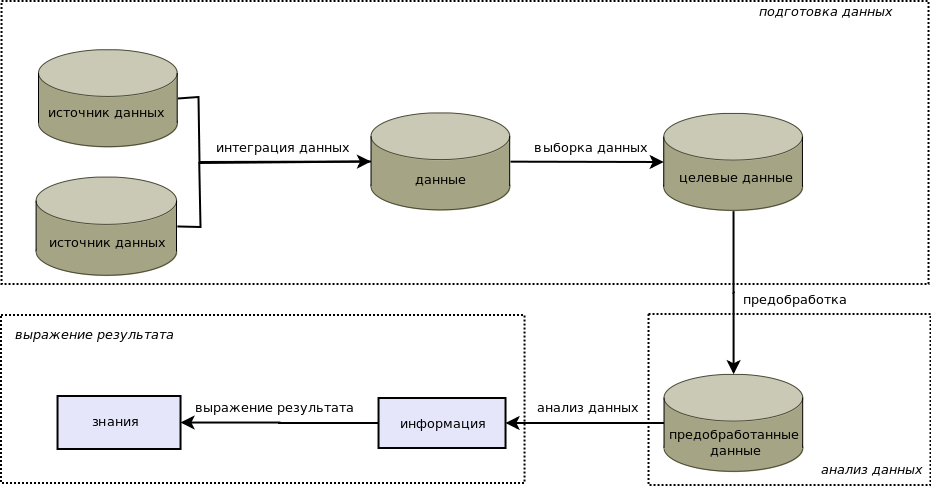
\includegraphics[scale=0.5]{datamining1.png}
	\caption{Основной процесс анализа данных}
	\label{pict:datamining1}
\end{figure}

Интеллектуальный анализ данных на основе нейронных сетей состоит из
подготовки данных, правила извлечения и оценивание правил, как показано на рис. \ref{pict:datamining2}

\begin{figure}[h!]
\center
	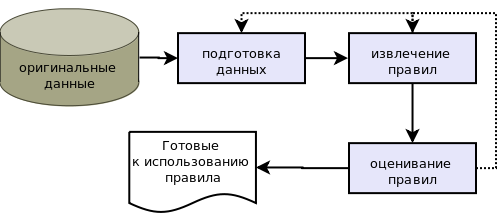
\includegraphics[scale=0.7]{datamining2.png}
	\caption{Процесс анализа данных, основанный на нейронной сети}
	\label{pict:datamining2}
\end{figure}

\begin{enumerate}
\item Подготовка данных.
Подготовка данных является определение и процесс интеллектуального анализа данных, чтобы
сделать его пригодным конкретного интеллектуального анализа данных методом. Подготовка данных является
первым важным шагом в интеллектуальном анализе данных и играет решающую роль
во всем процессе интеллектуального анализа данных. В основном включает в себя
следующие процессы:
\begin{enumerate}
\item Очистка данных. Устранение шумов данных и устранение несоответствия в данных.
\item Выборка данных. 
\item Предварительная обработка. 
\item Выражение данных. Выражение данных состоит в преобразовании после предварительной обработки
в форму, которая может быть принята алгоритмом интеллектуального анализа данных, основанном на нейронной сети. Интеллектуальный анализ данных на основе нейронной сети может работать только с числовыми данными, так что это необходимо трансформировать символьные данные в цифровые. Простейший метод заключается в создании таблицы с взаимно-однозначным соответствием между символьными данными и числовыми. 
\end{enumerate}
\item Извлечение правил;
\item Оценивание правил.
\end{enumerate}
Хотя цель оценки правил зависит от каждого конкретного применения, но, в общем случае, правила могут 
оцениваться по следующим критериям.
\begin{itemize}
\item найти оптимальную последовательность извлечения правил, что позволяет 
получать лучшие результаты на данном наборе данных;
\item проверить правильность извлечения правил;
\item определить, сколько знаний в нейронной сети не были извлечены;
\item обнаружить несоответствия между извлеченными правилами и обученной нейронной сетью.
\end{itemize}

Есть еще более серьезный принципиальный недостаток статистических пакетов, ограничивающий их применение в Data Mining. Большинство методов, входящих в состав пакетов опираются на статистическую парадигму, в которой главными фигурантами служат усредненные характеристики выборки. А эти характеристики, как указывалось выше, при исследовании реальных сложных жизненных феноменов часто являются фиктивными величинами. 

Существуют различные варианты применения нейронных сетей для анализа данных такие как  
интеллектуальный анализ данных на основе самоорганизующихся нейронных сетей и на основе нечеткой нейронной сети.
Самоорганизационный процесс - процесс обучения обучения без учителей. Исследуются 
важные характеристики или некоторые врожденные знания в группе данных, таких как
характеристики распределения или кластеризации в соответствии с определенной функцией;

Хотя нейронная сеть имеет сильные функции обучения, классификации, ассоциативной памяти, 
но в использовании нейронных сетей для интеллектуального анализа данных наибольшую трудность составляет то, что
 результаты на выходе не могут быть интуитивно понятны. 
 После введение нечеткой функции обработки в нейронную сеть, 
 она позволяет не только увеличить емкость продукционных выражений, но также система становится более стабильной. 
 Главным отличием от обычной нейронной сети является то, что в традиционной нейронной сети образцы могли принадлежать
одной категории. Нечеткие сети имеют способность отражать степень принадлежности.

Основные методы и подходы реализации:
\begin{itemize}
\item сочетание нейронной сети и интеллектуального анализа данных;
\item сочетание обработки знаний и нейронных вычислений;
Для оценки реализации алгоритма интеллектуального анализа данных
могут быть использованы следующие показатели и характеристики:
\begin{itemize}
\item качество моделирования в условиях шума и сырых данных;
\item модель должна быть понята пользователю и может быть использована для принятия решений;
\item модель может использовать знания для улучшения качества моделирования. 
Нейронные сети на самом деле можно рассматривать как черный ящик для пользователей, что делает процесс 
классификации и прогнозирования не понятым для пользователей и
невозможным для непосредственного использования для принятия решений.
\end{itemize}
\end{itemize}

Методы интеллектуального анализа данных.
Классические методами приобретения знаний из массивов данных являются статистические методы. 
В интеллектуальном анализе данных используются новые методы, кроме статистических. Эти методы имеют свое происхождение в области искусственного интеллекта. Они отличаются от классических статистических методов в следующим:
\begin{itemize}
\item ищут неизвестные и неожиданные отношения, которые могут быть обнаружены путем изучения данных в базе данных. Они пытаются найти в наборах данных такие закономерности, которые принесут пользователям новый взгляд в сфере интересов и позволят ему сформулировать новые гипотезы. Статистические методы используют несколько иной путь. Они проверяют или отвергают гипотезы заявленных априори.
\item Методы интеллектуального анализа данных можно использовать и в таких случаях, в которых 
использование классических статистических методов не подходит. Например, когда имеется большой объем 
многомерных данных  или когда не представляется возможным полагать, что данные имеют некоторое стандартное 
вероятностное распределение.
\end{itemize}
В интеллектуальном анализе данных изучаются и используются следующие методы получения знаний:
\begin{itemize}
\item статистические методы (прогноз временных рядов, кластерный анализ и др.);
\item продукционные правила ЕСЛИ. . . ТО;
\item деревья решений;
\item генетические алгоритмы;
\item нейронные сети.
\end{itemize}

Продукционные правила образуют базу знаний экспертной системы с продукционной архитектурой системы. При проектировании экспертной системы разработка продукционных правил является результатом обсуждения между инженером и группой экспертов.
 
 В интеллектуальном анализе данных изучаются методы автоматической разработки продукционных правил.
Такие методы в основном разработаны для создания правил называются ассоциативными правилами.
Целью правил ассоциации является выявление отношений между данными в больших базах данных, позволяют найти
элементы, которые предполагают наличие других элементов этой же серии.
Проблемы автоматического создания ассоциативных правил были интенсивно изучались в последнее десятилетие. 
Были разработан эффективные алгоритмы.

Дерево решений представляет возможным представление решения функцией. Оно используется, когда полное знание данных 
не является необходимым для принятия соответствующего решения, и когда процесс получения данных является затратным. Существуют алгоритмы для автоматического построения деревьев решений. Автоматическое построение деревьев решений является традиционной частью искусственного интеллекта.

Деревья решения являются одним из наиболее популярных подходов к решению задач Data Mining. Они создают иерархическую структуру классифицирующих правил типа <<ЕСЛИ... ТО...>> (if-then), имеющую вид дерева. Для принятия решения, к какому классу отнести некоторый объект или ситуацию, требуется ответить на вопросы, стоящие в узлах этого дерева, начиная с его корня. Вопросы имеют вид <<значение параметра A больше x?>>. Если ответ положительный, осуществляется переход к правому узлу следующего уровня, если отрицательный - то к левому узлу; затем снова следует вопрос, связанный с соответствующим узлом.

Популярность подхода связана как бы с наглядностью и понятностью. Но деревья решений принципиально не способны находить <<лучшие>> (наиболее полные и точные) правила в данных. Они реализуют наивный принцип последовательного просмотра признаков и <<цепляют>> фактически осколки настоящих закономерностей, создавая лишь иллюзию логического вывода.

Генетический алгоритм является универсальным методом для создания объектов с заданными свойствами.
Объекты описаны последовательностью символов, которая по своей форме аналогична геному живых организмов. Генетический
 алгоритм создает поколения объектов. Новое поколение возникает в результате мутации, кроссовера или их комбинация из
 этих объектов существующего поколения, которые имеют наибольшее значение фитнесс-функции. Эволюция моделируется
  генетическим алгоритмом, направленным на генерацию объектов с большим значением функция пригодности или, другими
  словами, объектов с заданными свойствами.
  
Генетические алгоритмы удобны тем, что их легко распараллеливать. Например, можно разбить поколение на несколько групп и работать с каждой из них независимо, обмениваясь время от времени несколькими хромосомами. Существуют также и другие методы распараллеливания генетических алгоритмов.

Генетические алгоритмы имеют ряд недостатков. Критерий отбора хромосом и используемые процедуры являются эвристическими и далеко не гарантируют нахождения <<лучшего>> решения. Как и в реальной жизни, эволюцию может <<заклинить>> на какой-либо непродуктивной ветви. И, наоборот, можно привести примеры, как два неперспективных родителя, которые будут исключены из эволюции генетическим алгоритмом, оказываются способными произвести высокоэффективного потомка. Это особенно становится заметно при решении высокоразмерных задач со сложными внутренними связями.

Самоорганизующиеся карты Кохонена стали многообещающим метод в кластерном анализе. Они адаптированы для обучения без учителя. Неконтролируемый процесса обучения в SOM может быть кратко описать следующим образом \ref{pict:kohonen}.
После процесса обучения, подобные наборы элементов активируют тот же нейрон. SOM делит входной набор на подмножества подобных записей. Таким образом, SOM представляет собой метод кластерного анализа и часто используется для удобного представления данных.

\begin{figure}[h!]
\center
	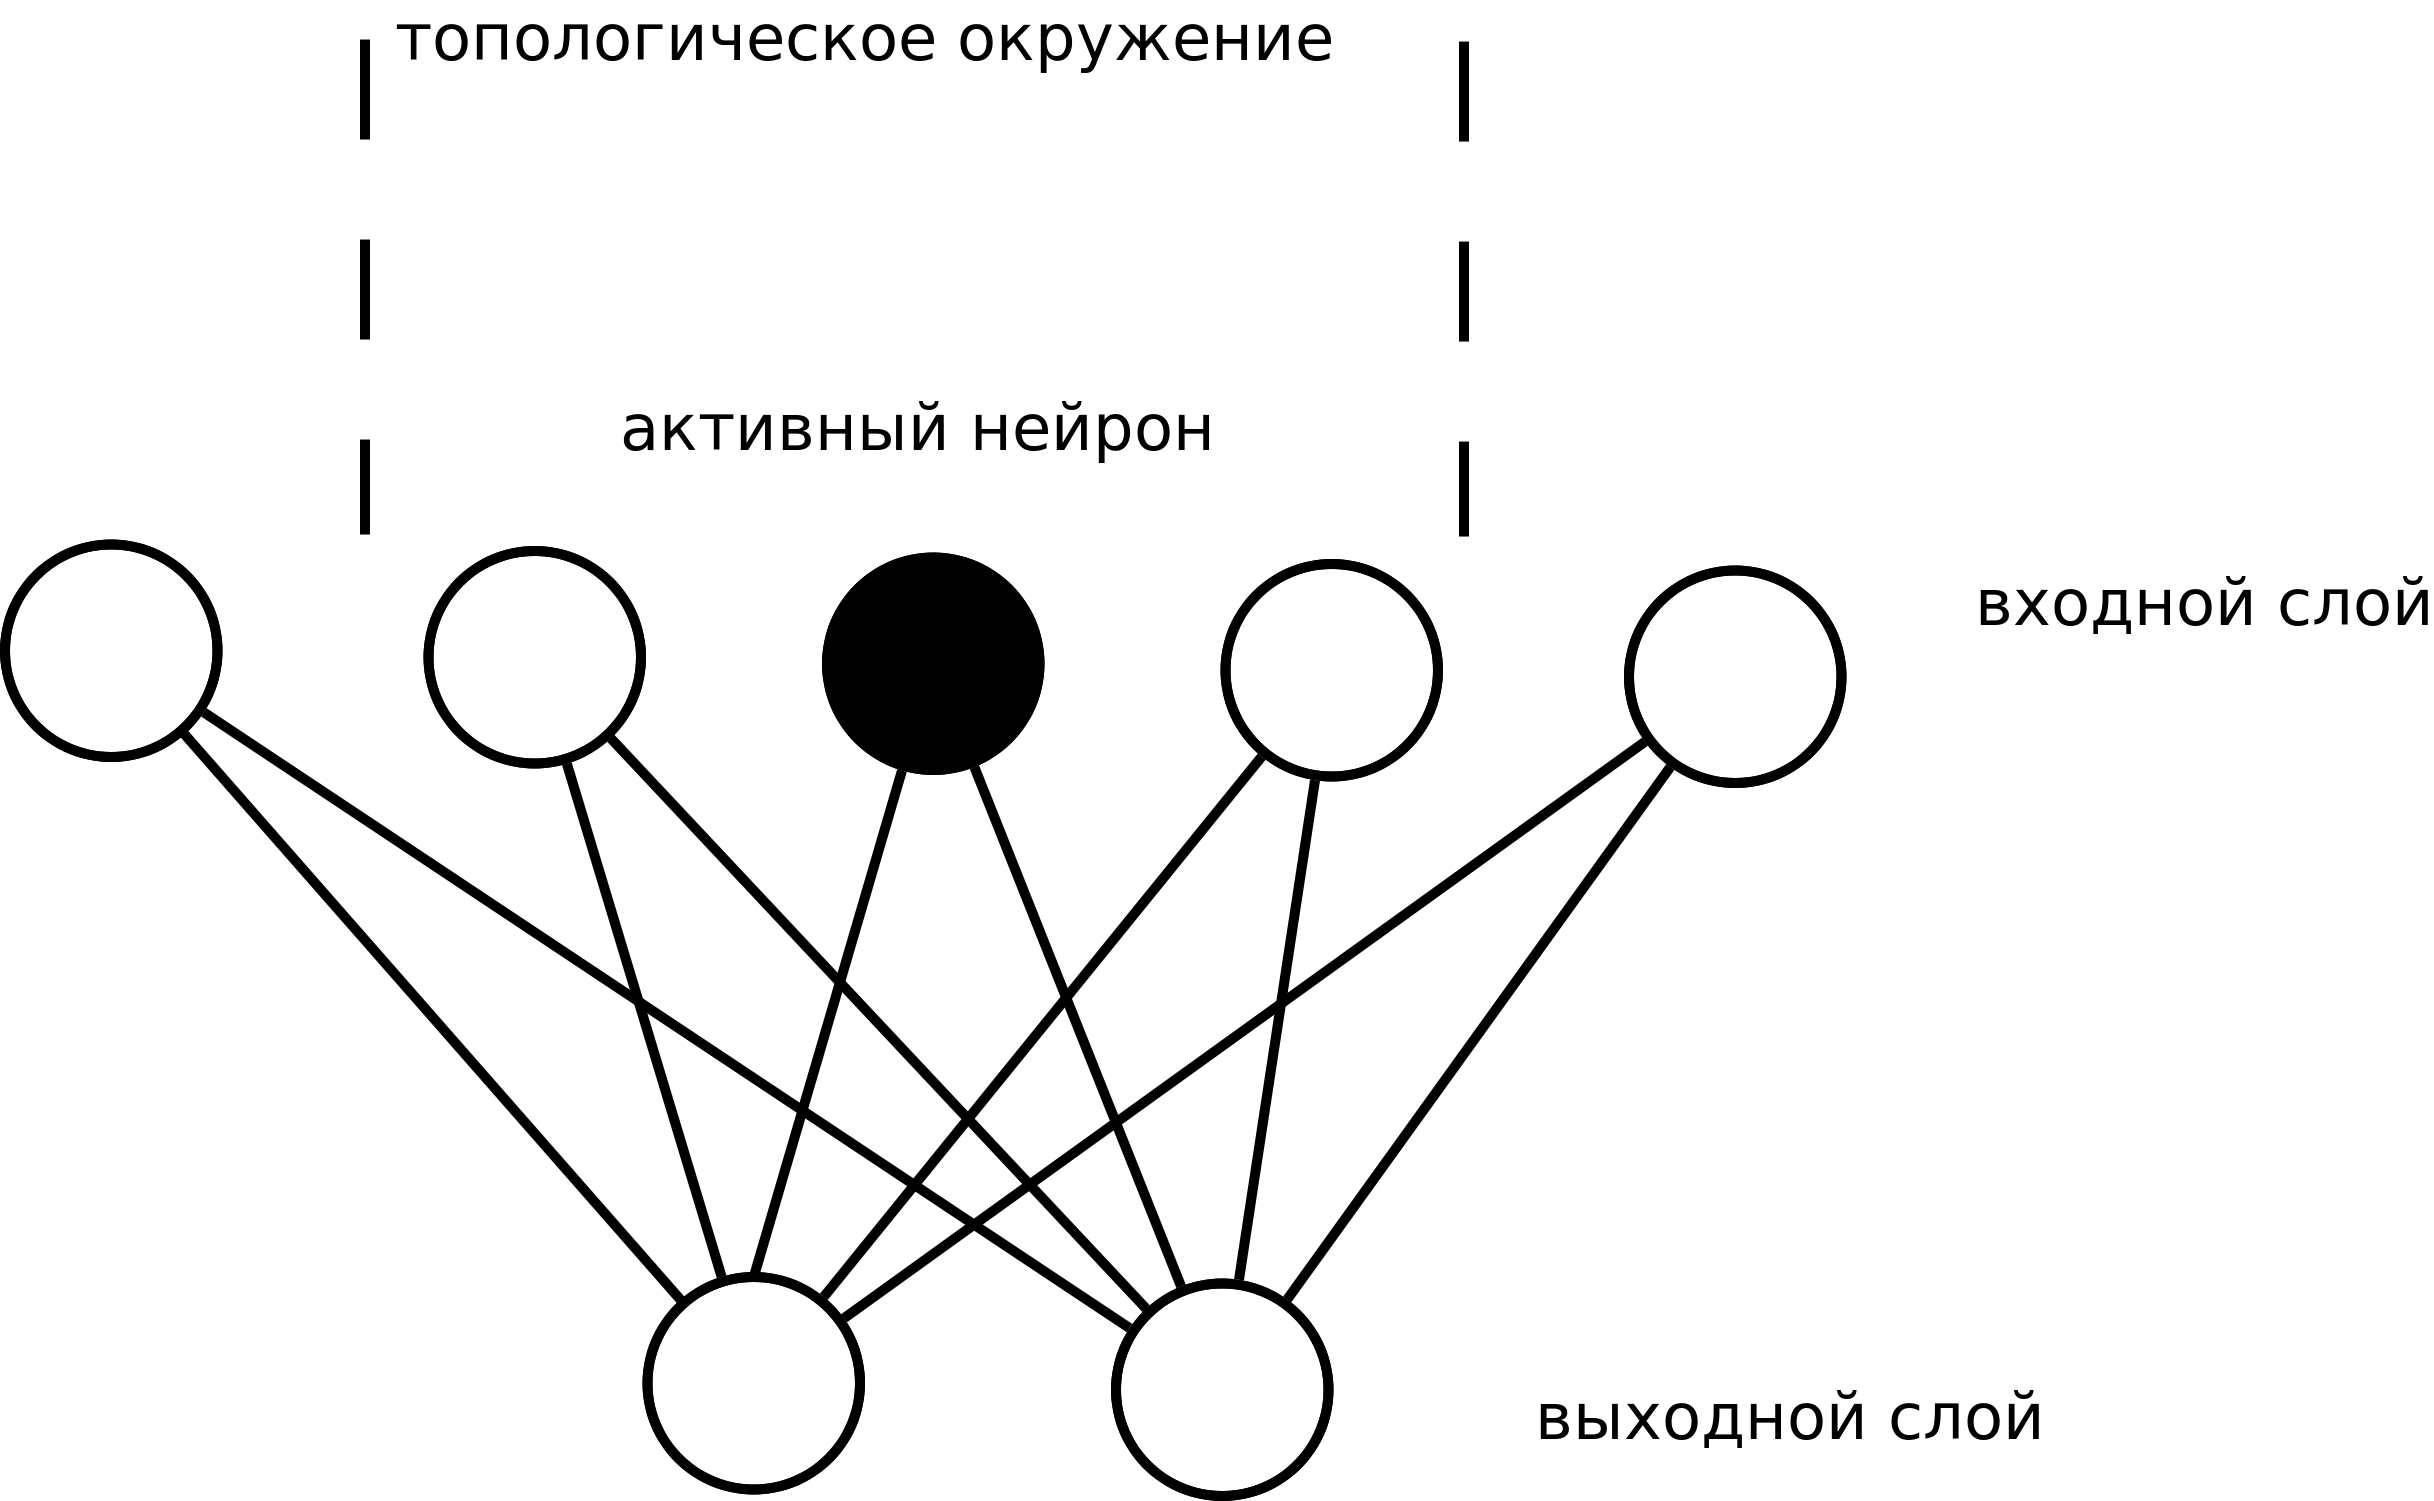
\includegraphics[width=140mm]{kohonen.png}
	\caption{Самоорганизующиеся карты кохонена}
	\label{pict:kohonen}
\end{figure}

В интеллектуальном анализе данных самоорганизующиеся карты Кохонена имеют следующие преимущества по сравнению со стандартными статистическими методами:

\begin{itemize}
\item Интеллектуальный анализ данных обычно имеет дело с многомерными данными. Запись в базе данных обычно состоит из большого количества элементов. Эти данные не имеют регулярного многомерного распределения и, следовательно, традиционные статистические методы имеют свои ограничения, не являются эффективными. SOM позволяет эффективно обрабатывать многомерные данные.
\item Самоорганизующиеся карты предоставляют средства для визуализации многомерных данных.
\end{itemize}

Основным недостатком нейросетевой парадигмы является необходимость иметь очень большой объем обучающей выборки. Другой существенный недостаток заключается в том, что даже натренированная нейронная сеть представляет собой черный ящик. Знания, зафиксированные как веса нескольких сотен межнейронных связей, совершенно не поддаются анализу и интерпретации человеком.

Анализ знаний - нетривиальный процесс. В настоящее время используется множество различных методов интеллектуального анализа данных. Методы анализа данных играют важную роль в управлении сложными системами, имеют большую область применения в экономике. Программное обеспечение, реализующее алгоритмы интеллектуального анализа данных, существуют на рынке, но в настоящее время цена на него высока. 

\section{Методы анализа рядов на основе нечетких систем}
Под нечетким временным рядом (НВР) будем понимать упорядоченную последовательность наблюдений над некоторым явлением, состояния которого изменяются во времени, если значение  состояния в момент $t_i$  выражено с помощью нечеткой метки
$\tilde{x_i} \in \tilde{X}, i \in [1, n]$,  $n$ – количество членов  ряда, то есть нечеткий временной ряд представим в виде 
\begin{equation}
\label{fuzzy_model_ts}
	\tilde{Y} = \lbrace t_i, \tilde{x_i} \rbrace 
\end{equation}   
где $\tilde{x_i}$ – $i$-тое нечеткое множество(нечеткая метка), $t_i$ – $i$-тое значение момента времени $t_1 \leq t_i \leq t_n$, $n$  – количество членов НВР. 

Нечеткая метка – это понятие на естественном языке, получаемое посредством фаззификации исходного четкого временного ряда. Таким образом, для каждому четкому элементу временного ряда соответствует пара $(X,\mu)$, где $X$ – лингвистическое понятие, $\mu$ – степень принадлежности элемента  указанному понятию.

Для описания развития моделируемого процесса в лингвистических терминах введем понятие временного ряда нечетких тенденций. Выделим далее базовые операции обработки нечетких тенденций. 

<<Нечеткой тенденцией (НТ) нечеткого временного ряда будем называть
нечеткую метку, выражающую характер изменения (систематическое движение)
 последовательности нечетких уровней НВР в заданном интервале времени.
Нечеткая тенденция выражает поведение НВР в лингвистическом виде, например:
 'Рост', 'Падение', 'Стабилизация', 'Колебания', 'Хаос'. Для нечетких
термов, обозначающих тенденцию, возможно применение модификаторов
'очень', 'более-менее' и т. д. Отметим важное свойство нечетких экспертных
оценок, обусловленное возможностью их ранжирования, что позволяет представить
 их совокупность в виде некоторой системы (шкалы) с отношениями.
Бинарные отношения, образованные на множестве нечетких экспертных оценок,
 порождают сравнительные оценки по различным критериям, такие, как
'Больше', 'Меньше', 'Примерно Равны', 'Рост', 'Падение', 'Предпочтительнее',
 'Лучше'. Такие сравнительные оценки представляют изменения
(различие) нечетких меток в различных пространствах: в пространстве объектов,
 во временном пространстве, в пространстве задач и характеризуют тенденции.
Изменения нечетких меток во временном пространстве порождают не-
четкий временной ряд с нечеткой тенденцией>>

<<В соответствии с логикой оценивания будем считать оценку нечеткого
уровня ВР - абсолютной нечеткой оценкой, а оценку изменения нечетких
уровней (нечеткую тенденцию) - сравнительной нечеткой оценкой>>.

В качестве инструмента как абсолютного, так и сравнительного нечеткого оценивания
Афанасьевой Т.В. была предложена специальная лингвистическая шкала - 
ACL-шкала (Absolute and Comparative Linguistic) [Афанасьева, 2008а]. 
<<Абсолютные оценки, полученные по ACL-шкале, соответствуют нечетким оценкам (меткам) уровней нечеткого временного ряда, а сравнительные оценки – нечетким тенденциям НВР>>.


В отличие от традиционного ВР значениями нечеткого ВР являются нечеткие множества, а не действительные числа наблюдений. В 1993 году Сонг и Чиссом(Song, Chissom) предложили модели стационарных и нестационарных (time-invariant и time-variant) нечетких временных рядов первого порядка (fist-order) и применили разработанные модели для прогнозирования количества регистрирующихся студентов университета штата Алабама, фаззифицировав предварительно четкий временной ряд. Это было первое определение моделей нечетких временных рядов. 

Пусть $X_t, (t=1,2,...) \subset R^1 $ - универсум, на котором определены нечеткие множества $y^i_t, (i=1,2,...)$ и $Y_t$ - коллекция $y_t^i, (i=1,2,...)$.Тогда $Y_t, (1,2,...)$ называется нечетким ВР.

На практике в большинстве ВР последовательные наблюдения зависимы, так, что:
\begin{equation}
	R= \lbrace (y_t, y_{t-1}), (y_{t-1}, y_{t-2}),... \rbrace \subseteq Y_t \times Y_{t-1}
\end{equation}
где $Y_t, Y_{t-1}$ обозначает переменные, а $y_t, y_{t-1}$ - наблюдаемые значения этих переменных. Наиболее частой моделью зависимости является явная функция отображения:
\begin{equation}
	f:Y_{t-1} \to Y_t
\end{equation} 
представленная линейной функцией (марковским процессом, модель AR):
\begin{equation}
	y_t = f (y_{t-1}, \phi, \epsilon) = \phi y_{t-1} + \epsilon
\end{equation}
где $\epsilon$ - случайная ошибка, шум.
В случае нечеткого ВР  в качестве модели авторегрессии используется нечеткое разностное уравнение:
\begin{equation}
	y_t^j = y_{t-1}^i \circ R_{ij}(t, t-1)
\end{equation}
$y_t^i \in Y_t, y_{t-1}^i \in Y_{t-1}, i \in I, j \in J, \circ - max min$,композиция, 
\begin{equation}
	R(t, t-1) = 	\bigcup_{ij} R_{ij}(t, t-1)
\end{equation}
есть система нечетких отношений, которая символически может быть записана в виде $Y_t \to Y_{t-1}$.
Систему отношений $R$ в выражении 
\begin{equation}
	Y_t = Y_{t-1} \circ R(t, t-1)
\end{equation}
называют моделью нечеткого ВР первого порядка, данная модель – важный частный случай общей модели порядка $p$:
\begin{equation}
	Y_t = (Y_{t-1} \times Y_{t-2} \times ... \times Y_{t-p}) \circ R(t, t-p),
\end{equation}

\begin{equation*}
	R(t, t-p)= \left. \begin{aligned}
	max \\
	p
\end{aligned} \right\{
\quad 
\left. \begin{aligned}
	min \\
	j, i_1, i_2,...,i_p
\end{aligned} \{y^j_t,y^{i_1}_{t-1},...,y^{i_p}_{t-p} \} \right \}
\quad 
\end{equation*}

Моделирование нечетких временных рядов (по Сонгу) состоит в реализации следующих шагов:
\begin{enumerate}
\item Фаззификация входных данных – разбиение данных на множество интервалов, определение лингвистических значений нечетких множеств и функций принадлежности.
\item Формирование логических отношений $Y_t \to Y_{t-1}$ и вычисление

 $R_{ij}(t,t-1)$ для каждой импликации.
\item Вычисление результирующего отношения $R$ как объединение 

$\bigcup_{i,j} R_{ij}(t,t-1) $
\item Применение полученной модели к входным данным и получение выходных результатов
\item Дефаззификация.
\end{enumerate}

Предложенная Сонгом модель НВР имеет следующие недостатки:
\begin{enumerate}
\item Требуется большое количество вычислений для определения нечеткого отношения.
\item Для определения нечеткой максиминной композиции модели, требуется большое количество вычислений, особенно, когда нечеткое отношение очень велико.
\item Точность предсказания не достаточна.
\item Отсутствие четких рекомендаций по выбору количества нечетких множеств, и определению интервалов их носителей. Данные задачи выполняются экспертом, и, как показывают исследования, от выбора интервалов сильно зависит результат исследования.
\item Проблема длин интервалов: различные длины интервалов могут привести к различным нечетким отношениям, и в свою очередь породить различные модели и результаты прогноза. 
\end{enumerate}

В задачах анализа тенденций НВР недостатки данной модели уменьшаются за счет большей размытости исходных данных и, следовательно, пониженным требованиям к точности. 